\documentclass[12pt]{article}

\usepackage[utf8]{inputenc}
\usepackage[T1]{fontenc}
\usepackage{xcolor}
\usepackage{fontawesome}
\usepackage[in]{fullpage} % narrower margins
\usepackage[sfdefault,light]{FiraSans}
\usepackage[normalem]{ulem}
\usepackage{graphicx}
\usepackage{lscape}

\renewcommand{\baselinestretch}{1.5} % increases space between lines
\newcommand\epita{\textsc{Épita}}
\newcommand\irill{\textsc{Irill}}
\newcommand\how{html\_of\_wiki}

\newcommand\asterismcolor{black!65}
\newcommand\asterism{\noindent\textcolor{\asterismcolor}{\small{$\phantom{x}_{*\,\,\,*}^{\,\,\,*}$}}}

\begin{document}
\noindent Valais Léo\\
\texttt{valais\_l}\\
20019

\bigskip

\begin{abstract}
  My \epita{} S7's internship has taken place at \textit{BeSport}, a startup
  developing a social network for sport fans and practitioners. It aims to be
  the most convenient and inclusive platform dedicated to sport. The objective
  is to support the every sport (popular or not) at any level---i.e., from local
  clubs to Olympic and international federations. BeSport counts about two
  dozens of employees---engineers, researchers, developers, data scientists,
  sport reporters, marketing and strategy experts.

  The whole stack---backend, frontend, iOS and Android applications---of BeSport
  is developed by making full use of the \textit{Ocsigen project}. It is a
  french research project, free and open source, first developed at the
  \irill{}\footnote{%
    L'Initiative pour la Recherche et l'Innovation sur le Logiciel Libre.
    It is a research laboratory created in 2010 by the famous computer science
    institute \textsc{Inria}, the Université Pierre-et-Marie-Curie and
    the Université Paris VII -- Diderot.
  } labs in 2006. I did not worked on the BeSport platform but
  instead for the Ocsigen project, as the startup is one of its main contributors.
  The other most important contributors are the Paris Diderot university and
  individuals from different high-tech companies such as Google or Jane Street.

  My mission was to redesign from scratch their documentation toolchain. My
  internship supervisor was Vincent Balat, head of the Ocsigen project,
  \textsc{Cto} at BeSport and computer science researcher. The documentation
  toolchain to be redesigned has gone through several iterations over the years.
  The very first version was made using \emph{Ocsimore}, a full-featured and
  generic online documentation manager. When it became obsolete (no one wanted
  to maintain it due to its complexity), a new, more specialized tool,
  \emph{\how} were developed to keep the Ocsigen documentation available online.
  However, that tool was not convenient at all. It was neither generic nor
  flexible at all. My contribution to Ocsigen was then to further simplify
  \how{}, making it easy to use, flexible and versatile.

  I worked essentially with Vincent Balat but many people were helpful giving me
  feedback and improvement ideas---Jérôme Vouillon (Ocsigen heavy contributor
  working at BeSport), BeSport developers (users of the documentation) and
  different Ocsigen maintainers who reviewed and criticized my work.

  The code base of \how{} have different origins and some parts are more than a
  decade old! (It means that the programming style is very different and that it
  contains many hacks now obsolete because of modern language features.) The
  very first expectation of my internship supervisor was to quickly be able to
  understand to code base for its most part. Since there my mission involved
  many modifications of existing code (sometimes with bugs), this first step was
  perhaps the most crucial one. Another very important requirement was to fully
  understand the important features to keep to upgrade the toolchain. Indeed, I
  had to work with years of documentations of many different projects, with
  different needs, maintainers and users. I also had to plan an effective
  deployment planning to \emph{smoothly} setup my solution for every project
  part of Ocsigen. More technically, I was expected to quickly master OCaml
  because I already worked with this family of languages before my internship.

  Ocsigen being an open-source project on GitHub, I was allowed to use my own
  laptop, which I did. I worked with the OCaml language, on GNU Emacs on Manjaro
  Archlinux. I used Travis CI to setup a \emph{Continuous Integration/Continuous
    Delivery} (CI/CD) environment for each project part of Ocsigen. I also wrote
  a little CSS, tested against the Firefox, Google Chrome, Opera and Apple
  Safari browsers.

  Figure \ref{fig:gantt} shows the timeline of my work.

  \begin{center}
  \asterism
  \end{center}

  My internship supervisor was mostly satisfied of my work, which turned out to
  be more complex and time consuming than initially thought. People in the team
  were nice for the most part and working condition were very good. Some Ocsigen
  contributors did not fully agreed on the design I choosed (with Vincent
  Balat's approval). Their critics were enlightening, constructive and most of
  the time valid. Fortunately, I addressed all the major issues that \how{} had
  before my internship. One contributor (which I have met only online) were a
  bit unpleasant but it is a detail since every other people I worked with were
  nice and interesting.

  The following list summarizes the engineering skills I acquired during my
  internship.
  \begin{itemize}
  \item Quick integration into an existing workflow.
  \item Strongly typed multi-paradigm language knowledge (OCaml).
  \item Understanding of complex needs.
  \item DevOp job (introduction).
  \item Deployment planning.
  \item Note taking.
  \item \textsc{Agile} methodology.
  \end{itemize}

  I am mostly satisfied with my internship experience: I met nice people,
  discovered the startup environment and its methodology, I contributed to an
  open-source research project and learned a lot. I learned about OCaml, had an
  introduction to the work of DevOp and lead a full deployment of my solution.
  The major negative point is
  that I was the only one to \emph{code} on the project. However, every line of
  code I wrote has been reviewed at least by my internship supervisor and every
  developer immediately answered every question I had.

  \begin{landscape}
  \begin{figure}[!h]
    \centering
    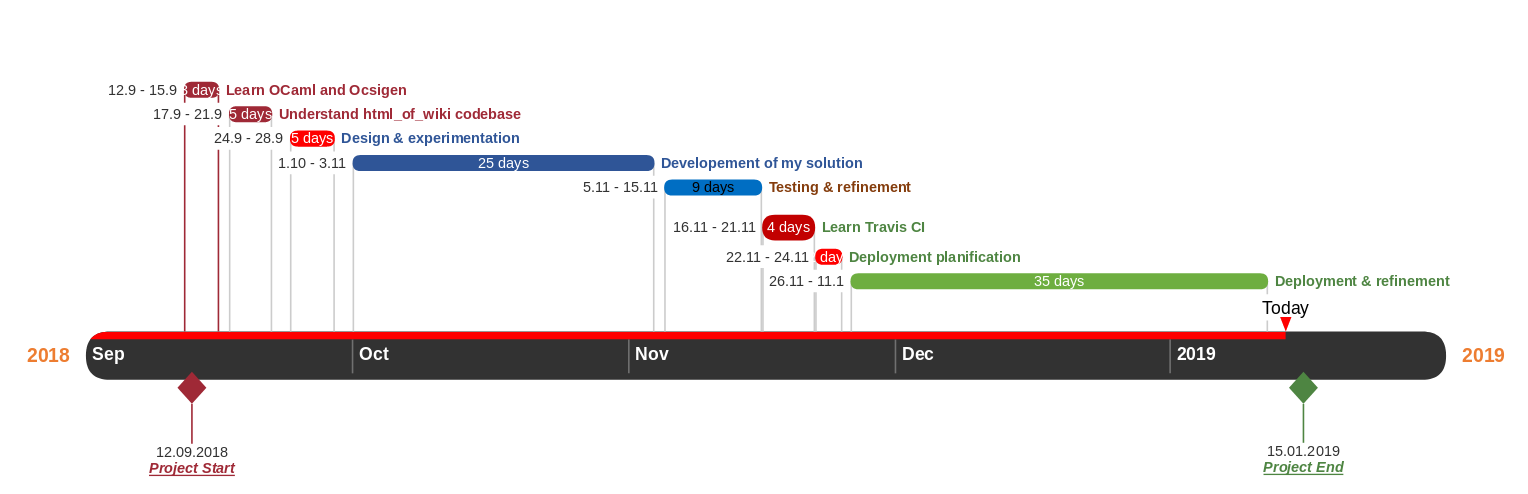
\includegraphics[scale=.45]{gantt.png}
    \caption{Project timeline}
    \label{fig:gantt}
  \end{figure}
  \end{landscape}
\end{abstract}
\end{document}